\section{Invariant Mass Reconstruction}

\subsection{Relativistic mass formula}

The key reconstructed observable is the invariant mass of the three-hadron B candidate. For a system of particles with total energy $E$ and total momentum $\vec{p}$, the invariant mass is defined by
\begin{equation}
  m^2 c^4 = E^2 - |\vec{p}|^2 c^2 .
\end{equation}
In high-energy-physics units with $c=1$, this becomes
\begin{equation}
  m^2 = E^2 - p_x^2 - p_y^2 - p_z^2 .
  \label{eq:invariant_mass}
\end{equation}

For each daughter track, the analysis uses a charged-kaon mass hypothesis,
\begin{equation}
  m_K = \SI{493.677}{\mega\electronvolt}/c^2 ,
\end{equation}
and reconstructs the energy as
\begin{equation}
  E_i = \sqrt{p_{x,i}^2 + p_{y,i}^2 + p_{z,i}^2 + m_K^2}.
\end{equation}
The B-candidate four-vector is then the sum of the three daughter four-vectors:
\begin{equation}
  E_B = \sum_{i=1}^{3} E_i, \qquad
  \vec{p}_B = \sum_{i=1}^{3} \vec{p}_i .
\end{equation}
Substituting these quantities into Eq.~\ref{eq:invariant_mass} gives the reconstructed B-candidate mass. The calculation is performed event-by-event with vectorised \texttt{numpy} operations.

\subsection{Mass spectrum before and after selection}

Figure~\ref{fig:mass_before} shows the reconstructed three-kaon mass spectrum before the baseline event selection. The distribution contains a broad combinatorial component as well as a visible accumulation near the expected B-meson mass region. This broad structure is typical of a preselection-level hadron-collider sample, where many random track combinations can satisfy a loose candidate definition.

\begin{figure}[H]
  \centering
  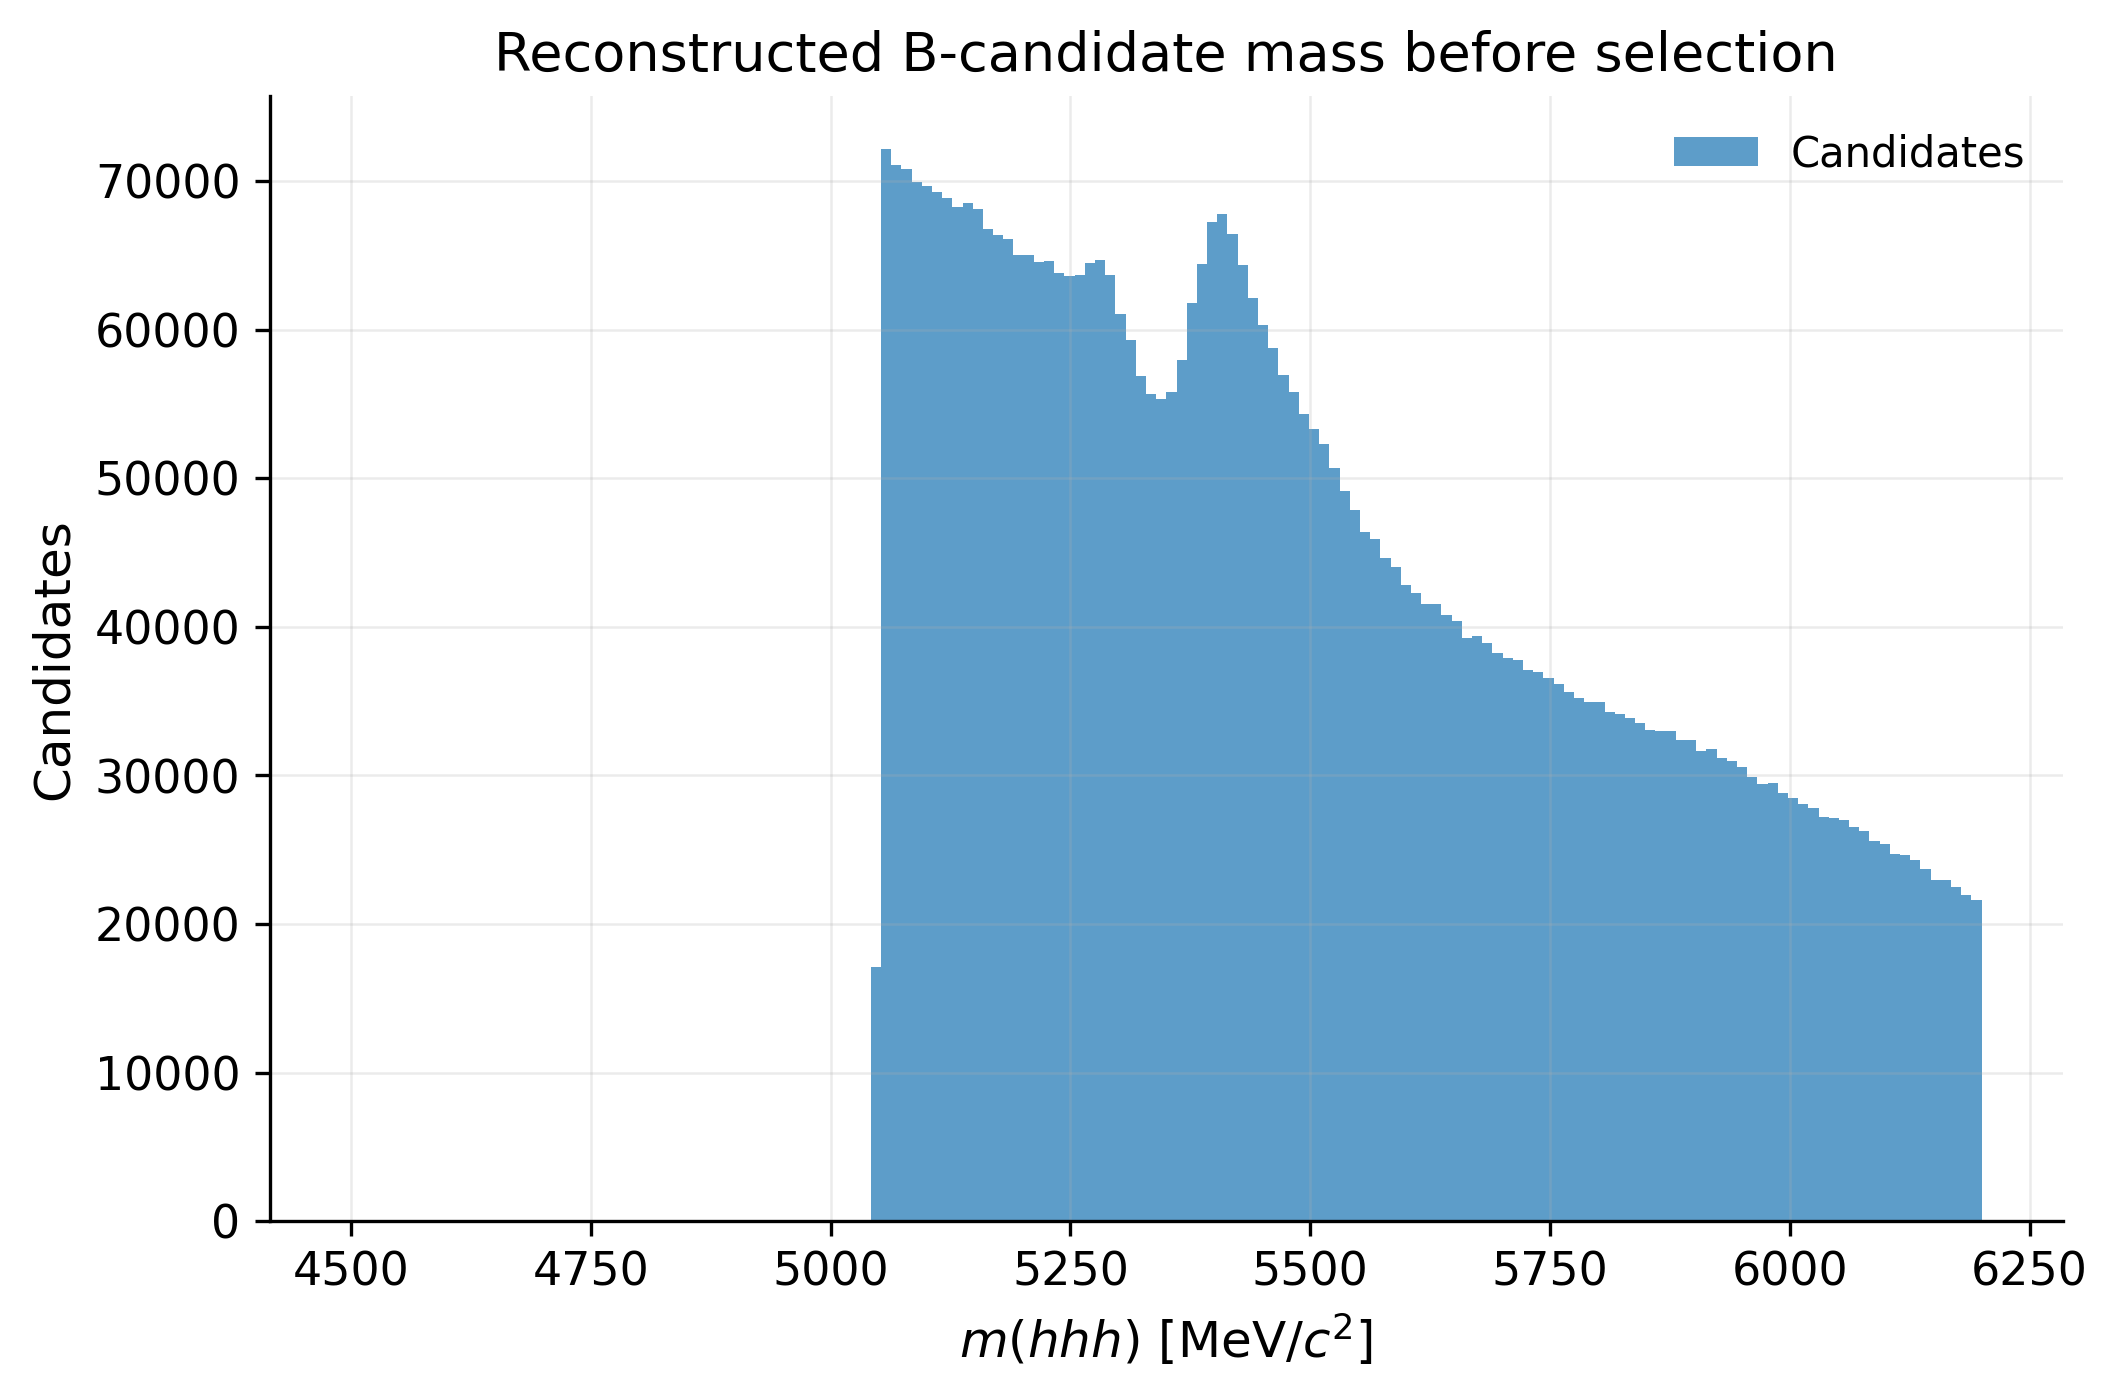
\includegraphics[width=0.82\textwidth]{B_mass_before_cuts.png}
  \caption{Reconstructed B-candidate invariant-mass distribution before baseline selection.}
  \label{fig:mass_before}
\end{figure}

After applying quality, displacement, and kaon-PID selections, the mass spectrum becomes visibly cleaner, as shown in Fig.~\ref{fig:mass_after}. The selection enhances the relative contribution of candidates compatible with a displaced B decay and suppresses a large fraction of combinatorial background.

\begin{figure}[H]
  \centering
  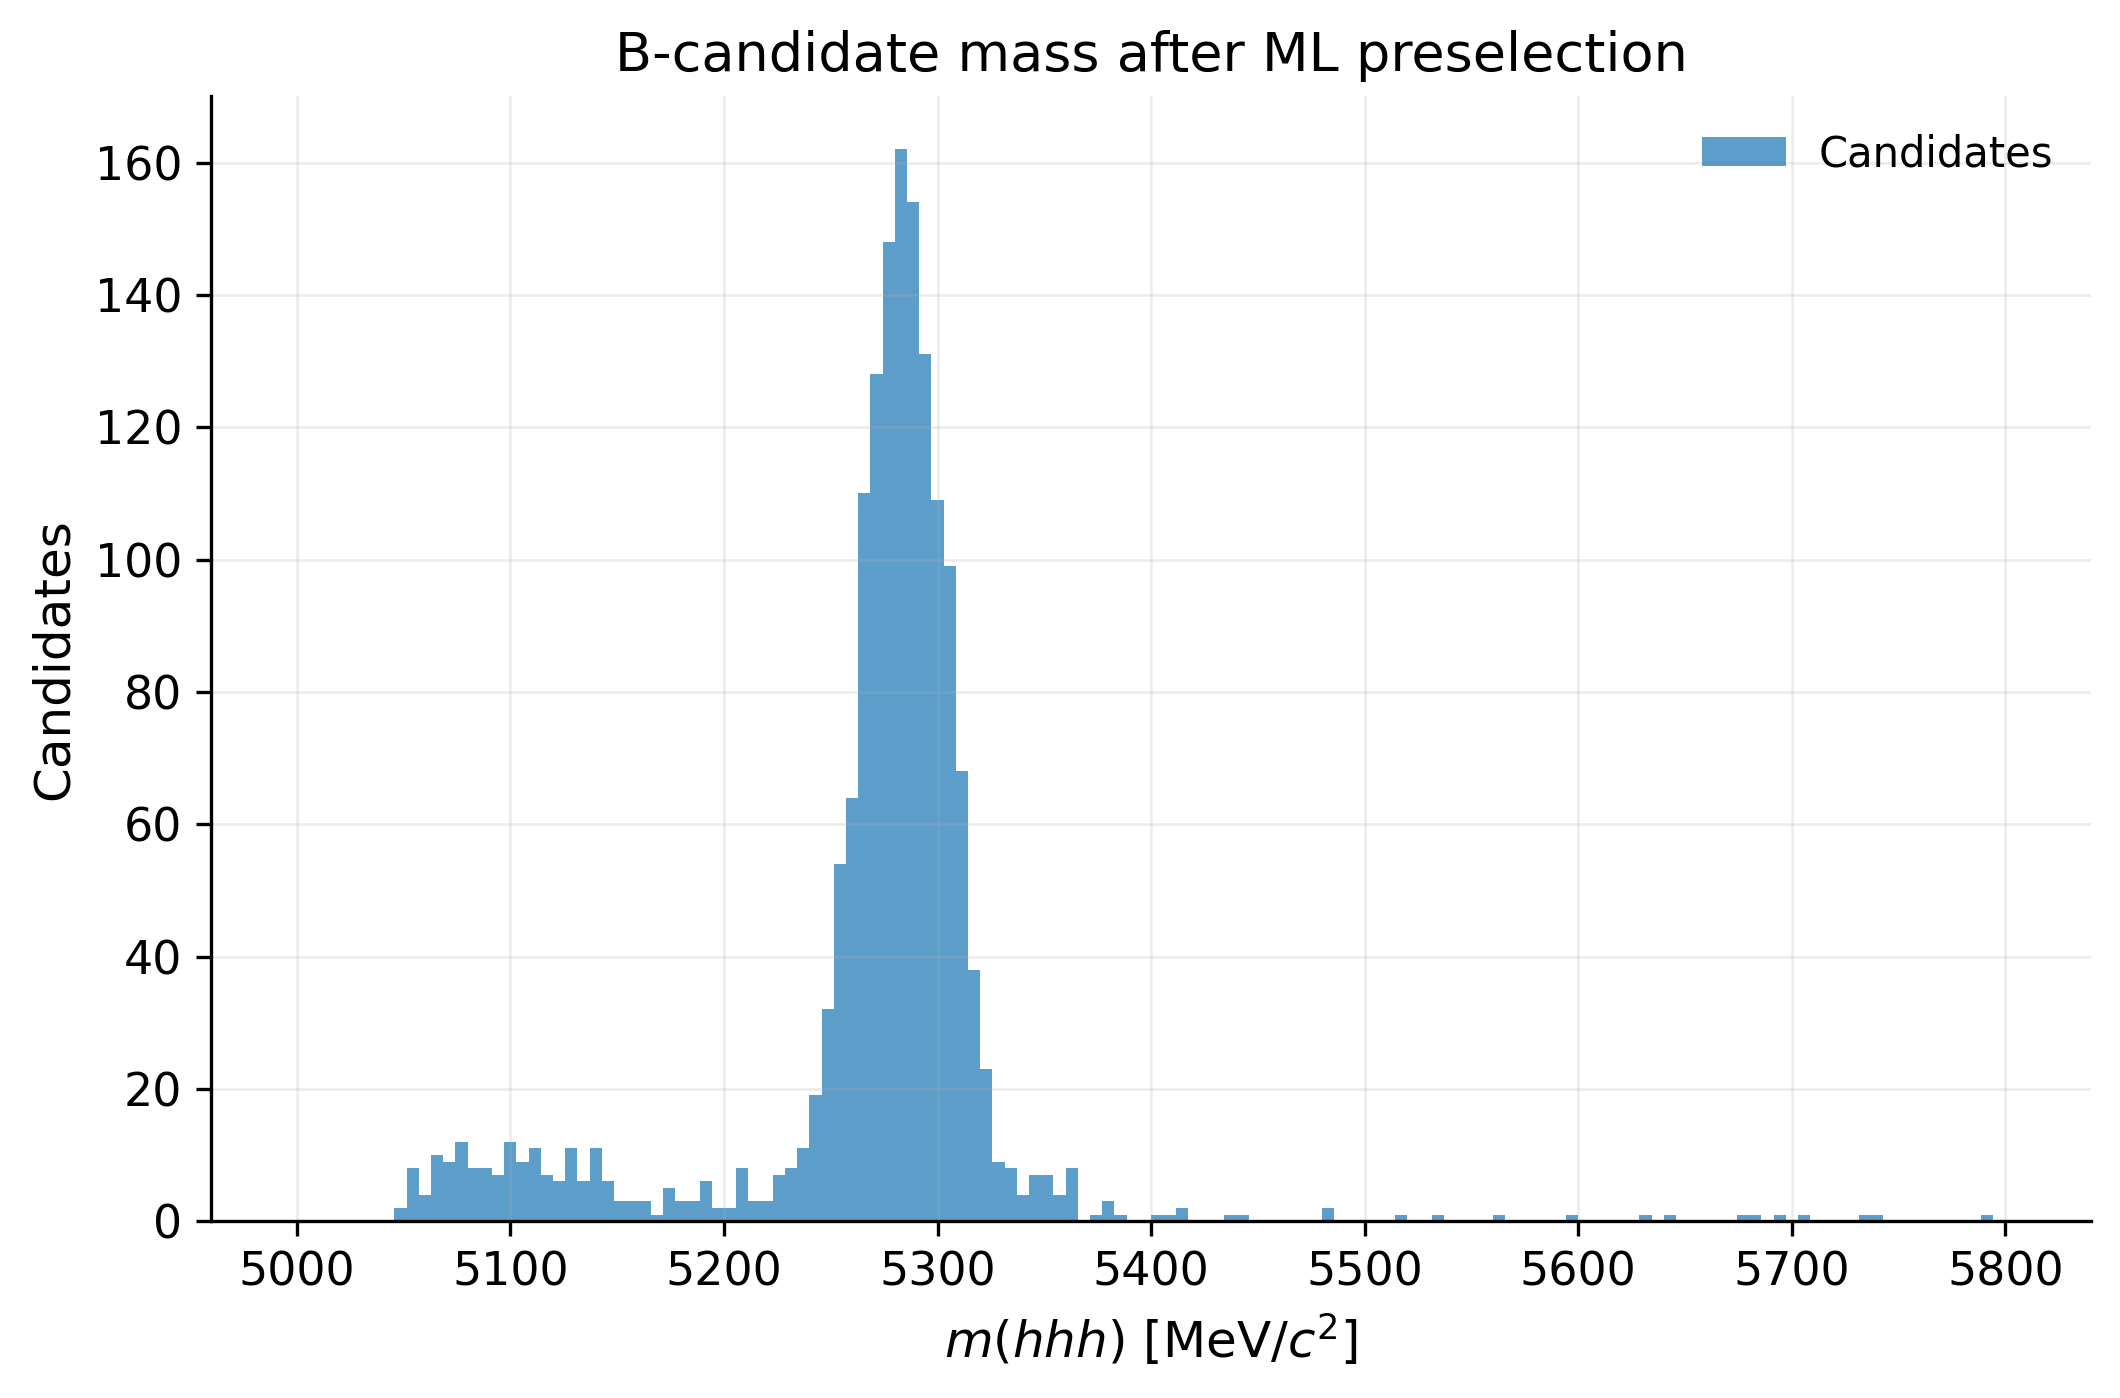
\includegraphics[width=0.82\textwidth]{B_mass_after_cuts.png}
  \caption{Reconstructed B-candidate invariant-mass distribution after baseline physics selections.}
  \label{fig:mass_after}
\end{figure}

\subsection{Signal-plus-background fit}
\label{sec:mass_fit}

A nominal signal extraction is performed with an extended binned maximum-likelihood
fit of the model
\begin{equation}
  f(m) =
  N_s S(m) + N_b B(m) ,
  \label{eq:mass_fit_model}
\end{equation}
where $S(m)$ is the signal mass shape, $B(m)$ a finite-range exponential
describing the combinatorial background, and $N_s$ and $N_b$ the fitted yields
inside the fitted interval. The likelihood is minimised with
\textsc{Minuit}~\cite{minuit} through the \texttt{iminuit} interface.

Two choices define the nominal configuration, and both are worth stating
explicitly because they are where this analysis is most fragile.

\paragraph{Fitted interval.} The fit is performed over
$5200 < m(hhh) < 5600~\mevcc$. The ntuple itself starts at $5050~\mevcc$, and
the spectrum between $5050$ and about $5180~\mevcc$ holds a structure that the
combinatorial background model does not describe. It is the same for the two
charges, and it falls off at the kinematic limit $m_B - m_\pi \approx
5140~\mevcc$ of a $B$ decay in which a pion is not reconstructed, smeared by the
resolution: the signature of partially reconstructed decays. An ARGUS shape with
that endpoint, convolved with the resolution, was tried over the full
$5050$--$5600~\mevcc$ range, but the ntuple boundary leaves only the top of the
shape visible and its curvature runs to the limit of its allowed range. Starting
the fit at $5200~\mevcc$ removes the region at the cost of a shorter low-mass
sideband.

\paragraph{Signal shape.} The nominal signal shape is a single Gaussian. A
common-mean double Gaussian was tested as the nominal shape, since detector-level
mass peaks often show a narrow core with broader tails, but on this sample its
wide component, $\sigma = 55 \pm 10~\mevcc$, takes over the combinatorial
background: the fitted background yield falls from $180 \pm 21$ to $63 \pm 39$
candidates, and the uncertainty on the signal yield inflates from $52$ to $63$.
The fit does reach a valid minimum, with a narrow-core fraction of
$0.91 \pm 0.03$, once several starting points are tried, but with a truncated
low-mass sideband the data cannot tell a broad resolution tail from the
background. The double Gaussian is therefore used as a systematic variation
rather than as the nominal shape.

The nominal fit of all selected candidates, both charges and both polarities
together, is shown in Fig.~\ref{fig:mass_fit}. Of the $2939$ selected candidates
($1645$ MagnetDown, $1294$ MagnetUp), $2573$ fall inside the fitted interval. The
results are
\begin{align}
  N_s &= 2394 \pm 52, \\
  N_b &= 180 \pm 21, \\
  \mu &= 5284.7 \pm 0.4~\mevcc, \\
  \sigma &= 19.5 \pm 0.4~\mevcc,
\end{align}
with $\chi^2/\mathrm{ndof}=0.74$. Fitted separately, the two polarities give the
same peak position and resolution within $0.1~\mevcc$. The fitted peak position lies within a few
$\mevcc$ of the known $B^\pm$ mass~\cite{pdg}, which is the main closure check on
the four-vector reconstruction and the mass hypothesis. The fitted resolution is
a detector resolution convolved with the kaon mass hypothesis, not a measurement
of the natural width.

\begin{figure}[H]
  \centering
  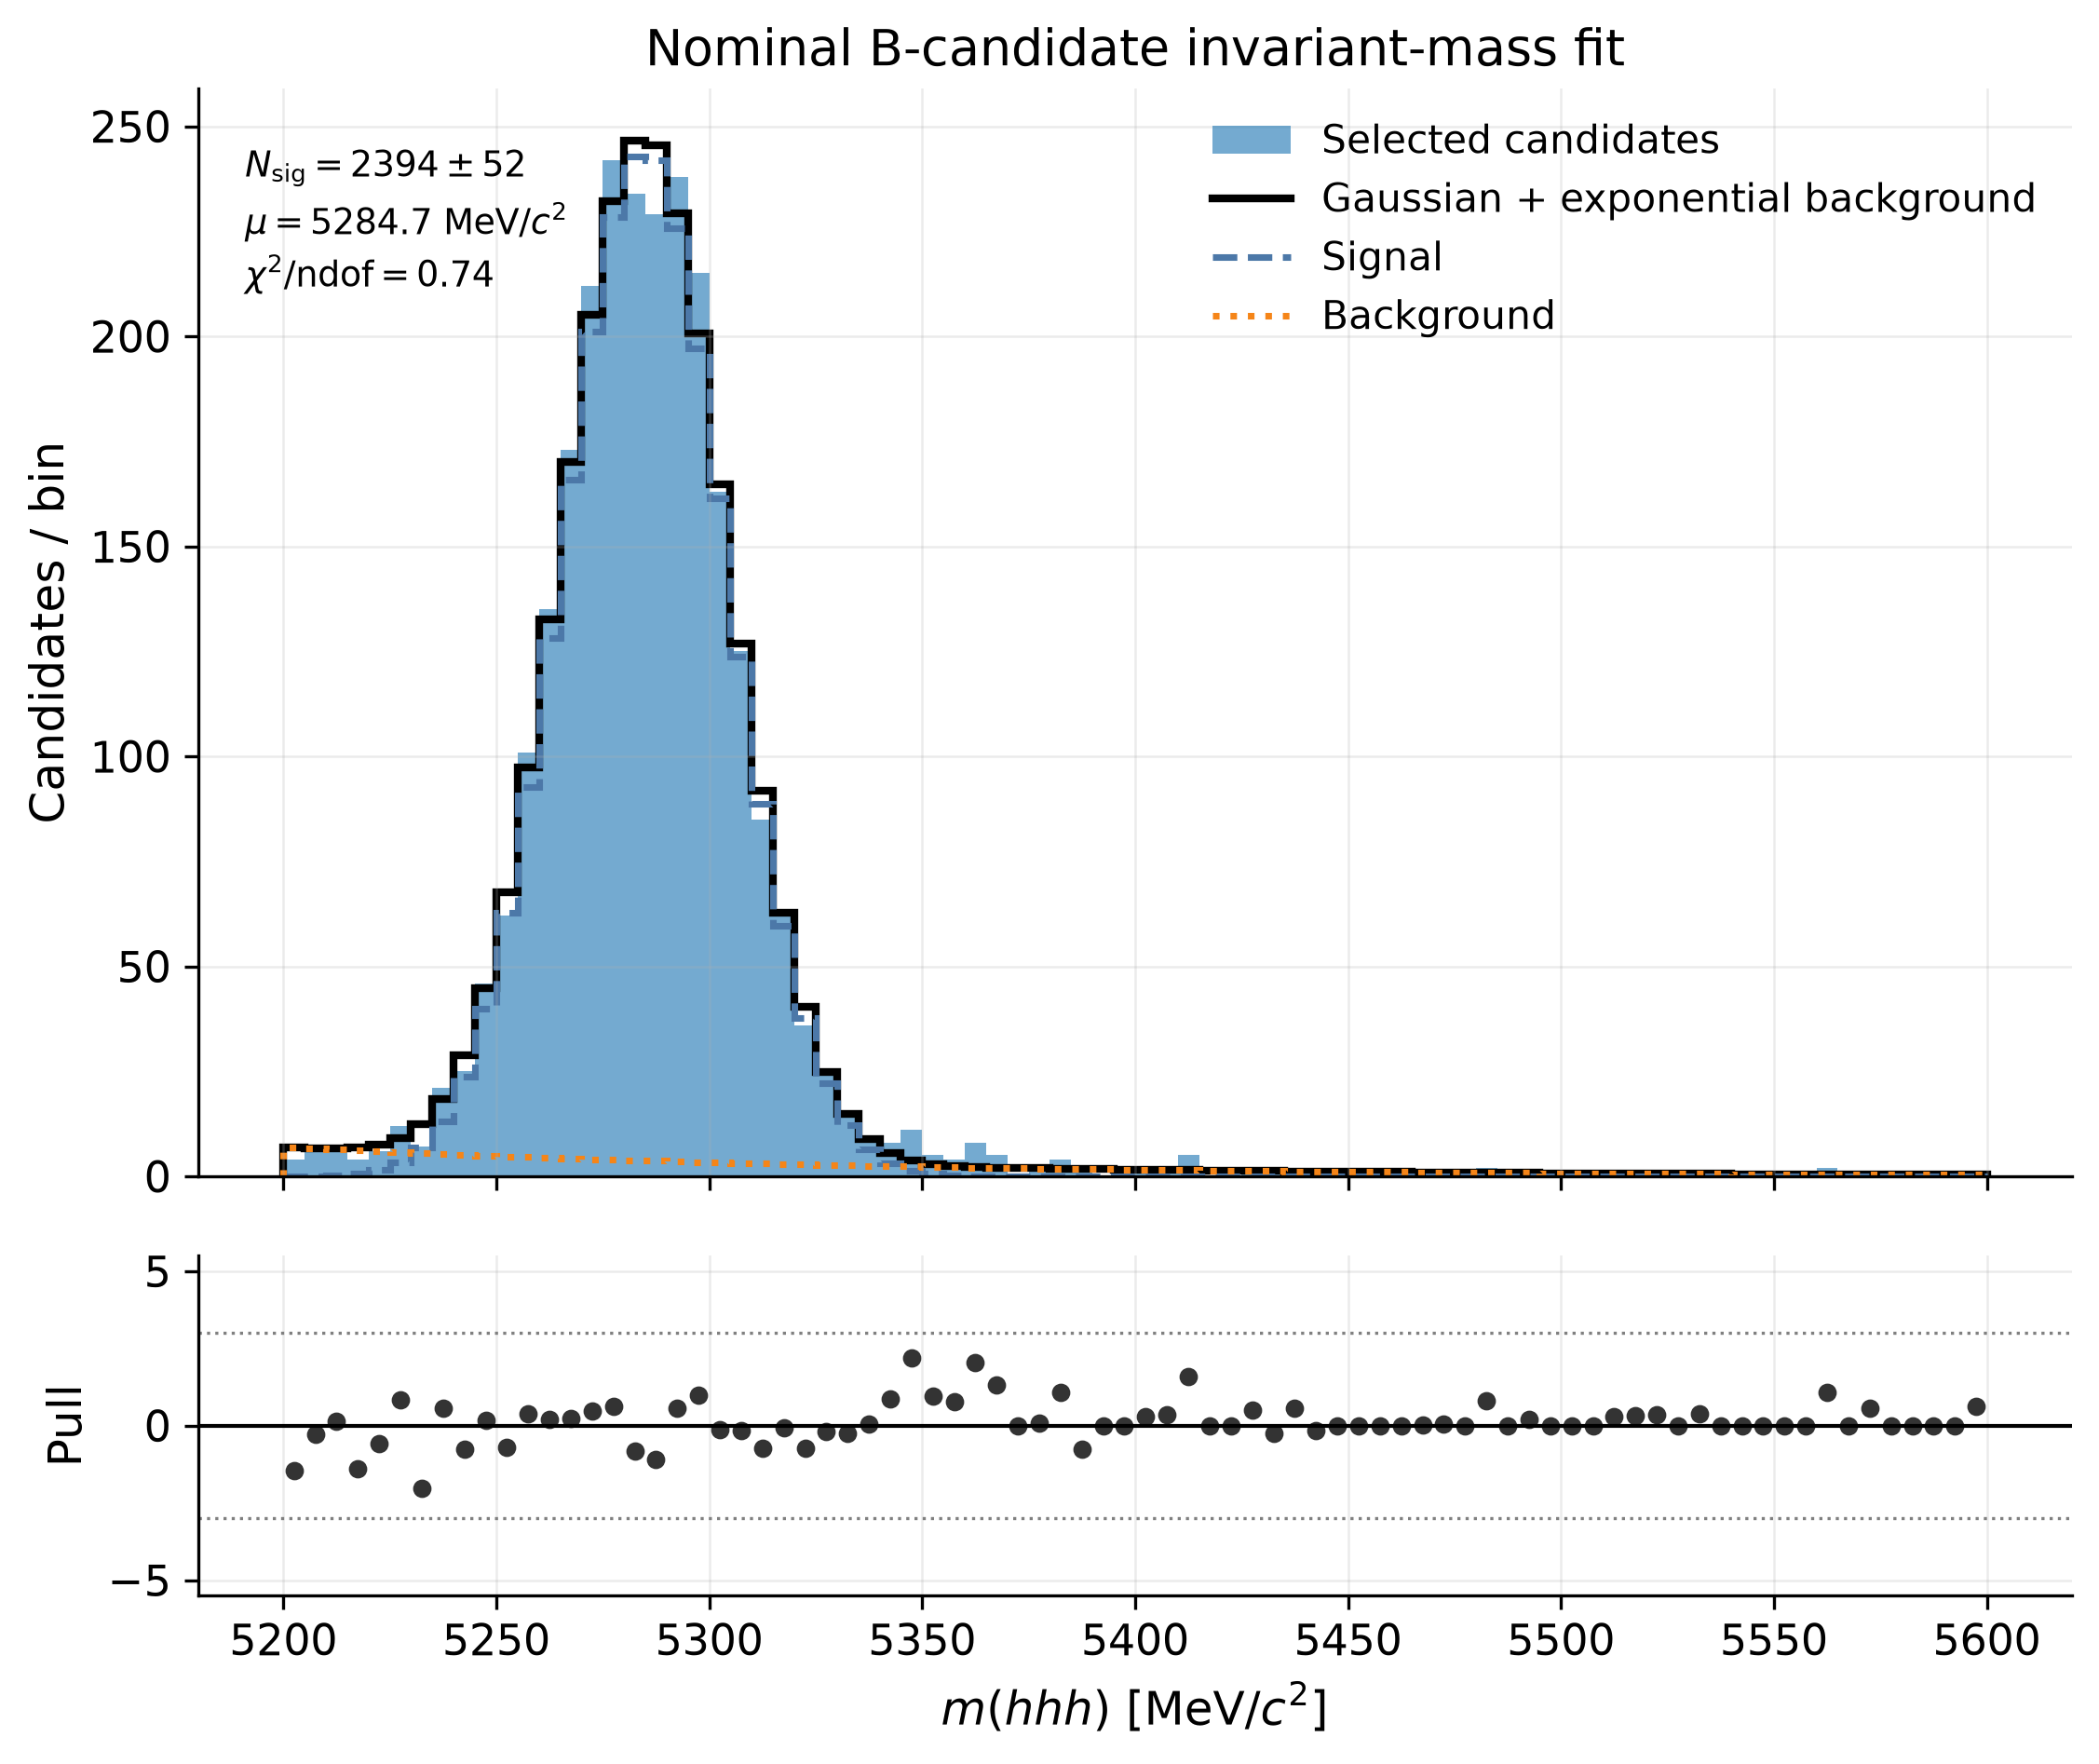
\includegraphics[width=0.82\textwidth]{mass_fit_plot.png}
  \caption{Selected $B$-candidate mass spectrum fitted with a single-Gaussian signal component and a finite-range exponential background, with fit residuals below.}
  \label{fig:mass_fit}
\end{figure}
